\documentclass[11pt,letterpaper]{article}
\usepackage{amsmath}
\usepackage{amsfonts}
\usepackage{amssymb}
\usepackage{fullpage}
\usepackage{graphicx}
\usepackage[normalem]{ulem}
\usepackage{url}

\begin{document}

\begin{center}
\huge
\textsc{Smart Refrigerator Design Project}\\
\Large
\textsc{Progress Report III} \\
\vspace{.20cm}
\hrule
\vspace{.40cm}
\normalsize
Steven Strapp, Ben Reeves, Dustin Stroup \\
\today \\
\vspace{1cm}
\end{center}

\section{Updated Milestone Chart}
\begin{table}[h!]
\begin{center}
\begin{tabular}{| p{3.5 cm} | p{2 cm} | p{2 cm}| p{2 cm} | p{6 cm} | }
\hline
\textbf{Milestone} & \textbf{Scheduled Date} & \textbf{Assigned} & \textbf{Modified Date} & \textbf{Comments} \\
\hline
BeagleBoard \newline procured & February 10, 2012 & SS & NA & Complete \\
\hline
Angstrom operating system running on board & February 24, 2012 & DS & NA & Complete \\
\hline
Peripherals properly interfacing with \newline board & March 02, \newline 2012 & DS & March 30, \newline 2012 & Complete aside from temperature sensor. Was not considered in \newline original timeline. \\
\hline
Basic mobile UI, \newline suitable for \newline debugging & March 09, \newline 2012 & BR & NA & Complete \\
\hline
Basic base station UI, suitable for \newline debugging & March 09, \newline 2012 &SS & NA & Completed basic GUI functionality. Incorporating duplicate item \newline support and databases. \\
\hline
Database I/O \newline configured & March 16, \newline 2012 & DS &  March 23, \newline 2012 & MySQL databases configured, can be accessed with Python \newline application. \\
\hline
Testing and \newline integration of \newline temperature and \newline humidity sensor & March 16,  \newline 2012 &SS & March 30, \newline 2012 & Partially complete. Tested using Arduino. Beagleboard GPIO \newline interface configured, needs testing. \\
\hline
Database and web server hosted by\newline Beagleboard & March 16, \newline 2012 & DS & NA & Running, web server functionality needs to be incorporated. Mobile app will access SQL databases directly, purpose of web server \newline becoming unclear.\\
\hline
Beagleboard \newline touchscreen display procured & March 16, \newline 2012 & DS & NA & Still awaiting delivery. \\
\hline

\end{tabular}
\end{center}
\end{table}

\begin{table}[h!]
\begin{center}
\begin{tabular}{| p{3.5 cm} | p{2 cm} | p{2 cm}| p{2 cm} | p{6 cm} | }
\hline
\textbf{Milestone} & \textbf{Scheduled Date} & \textbf{Assigned} & \textbf{Modified Date} & \textbf{Comments} \\
\hline
Mobile application integrated with web server & March 30, \newline 2012 &BR & April 6, \newline 2012 & Database integration still required.\\
\hline
User profiling and statistical analysis & March 30,\newline 2012 & SS & April 6, \newline 2012 & Pushed out a week in favor of completing GUI front end and handling duplicate items.\\
\hline 
Shopping lists, item modification, basic \newline settings & March 30, \newline2012 & DS / SS & & Complete - SS. Added context \newline menus and hidden ``administrator" panel. \\
\hline
Updated base station UI & April 6,\newline 2012 & SS & & Complete, awaiting review by team or outside testers.\\
\hline
Updated mobile application & April 6, \newline2012 & BR & & \\
\hline
Improved robustness of mobile interface& April 13,\newline 2012 & DS & & \\
\hline
Integration testing \newline and system \newline verification & April 13, \newline2012 & BR & & \\
\hline
System testing and demo preparation & April 20, \newline2012 & SS & & \\
\hline
\end{tabular}
\label {MilestoneTable}
\end{center}
\end{table}

\quad \newline \quad
\quad \newline \quad
\quad \newline \quad
\quad \newline \quad

\pagebreak[4]

\section{Current Milestones}
\begin{table}[h!]
\begin{center}
\begin{tabular}{| p{3.5 cm} | p{2 cm} | p{2 cm}| p{2 cm} | p{6 cm} | }
\hline
\textbf{Milestone} & \textbf{Scheduled Date} & \textbf{Assigned} & \textbf{Modified Date} & \textbf{Comments} \\
\hline
Mobile application integrated with web server & March 30, \newline 2012 &BR & April 6, \newline 2012 & Database integration still required.\\
\hline
User profiling and statistical analysis & March 30,\newline 2012 & SS & April 6, \newline 2012 & Pushed out a week in favor of completing GUI front end and handling duplicate items.\\
\hline
Shopping lists, item modification, basic \newline settings & March 30, \newline2012 & DS / SS & & Complete - SS. Added context \newline menus and hidden ``administrator" panel. \\
\hline
Peripherals properly interfacing with \newline board & March \newline 02, 2012 & DS & March \newline 30, 2012 & Complete aside from temperature sensor. Was not considered in \newline original timeline. Beagleboard \newline GPIO  interface configured, \newline needs testing. \\
\hline
\end{tabular}
\end{center}
\end{table}

\section{Next Milestones}
\begin{table}[h!]
\begin{center}
\begin{tabular}{| p{3.5 cm} | p{2 cm} | p{2 cm}| p{2 cm} | p{6 cm} | }
\hline
User profiling and statistical analysis & March 30,\newline 2012 & SS & April 6, \newline 2012 & Pushed out a week in favor of completing GUI front end and handling duplicate items.\\
\hline
Updated mobile application & April 6, \newline2012 & BR & & \\
\hline
Improved robustness of mobile interface& April 13,\newline 2012 & DS & &  Also development of web interface? \\
\hline
\end{tabular}
\end{center}
\end{table}

\section{Status}
\begin{itemize}
\item Base station front end is nearly complete, and it awaiting peer review and testing by outside users.
\item The shopping list prediction algorithm is the only large remaining base station task.
\item The mobile interface needs to be completed and integrated with the MySQL databases.
\item Completing the base station code has produced an updated database schema as a side effect. The schema appears to be finalized.
\item GPIO interface has been configured, but needs testing with the actual temperature sensor. The hooks have been placed in base station code to poll the sensor.
\end{itemize}

\section{Gantt Chart}
\begin{figure}[h!]
\begin{center}
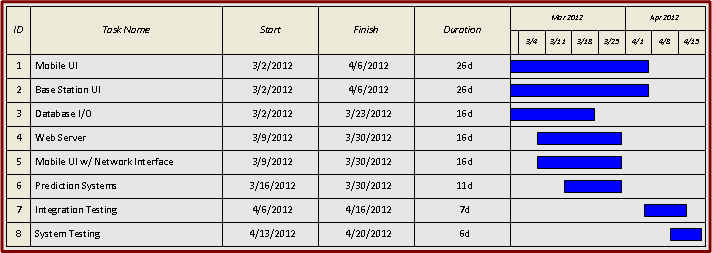
\includegraphics[scale=.6]{GanttChartI}
\end{center}
\end{figure}

\end{document}
